% !TeX root = ../../thesis.tex

\section{Security}

% https://learn.microsoft.com/en-us/windows/whats-new/windows-11-overview#security-and-scanning
% \subsection{User Access Control (UAC)}
% https://learn.microsoft.com/en-us/windows/security/identity-protection/user-account-control/how-user-account-control-works

\begin{figure}[htb]
    \centering
    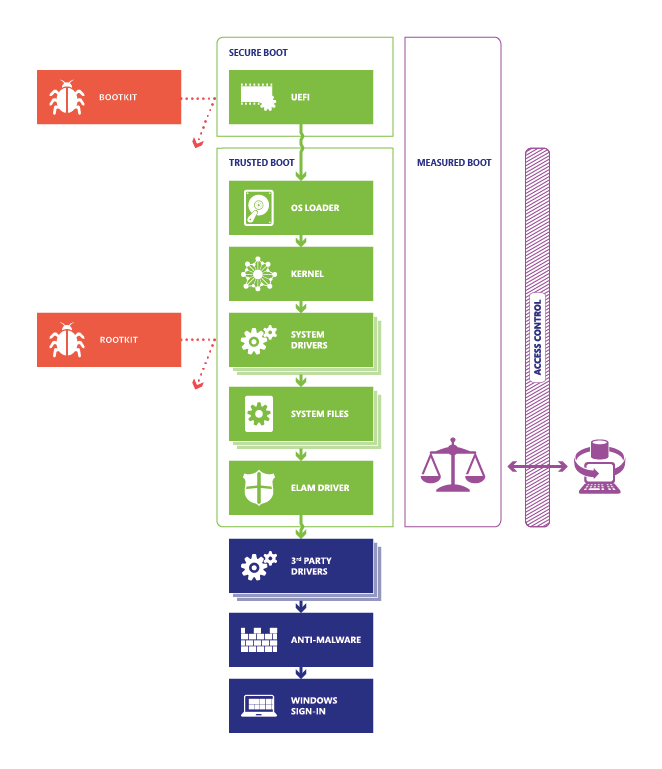
\includegraphics[width=1.0\textwidth]{windows/windows_startup_process.png}
    \caption{Windows startup process \cite{microsoft-secure-the-windows-boot-process}}
    \label{fig:windows-startup-process}
\end{figure}

\subsection{Secure Boot}

% https://learn.microsoft.com/en-us/windows-hardware/design/device-experiences/OEM-highly-secure-11

% https://learn.microsoft.com/en-us/windows/security/information-protection/secure-the-windows-10-boot-process#secure-boot
% All x86-based Certified For Windows PCs must meet several requirements related to Secure Boot:

% They must have Secure Boot enabled by default.
% They must trust Microsoft's certificate (and thus any bootloader Microsoft has signed).
% They must allow the user to configure Secure Boot to trust other bootloaders.
% They must allow the user to completely disable Secure Boot.

% Secure Boot to be enabled and configured to distrust the Microsoft 3rd Party UEFI CA signature, by default, to provide customers with the most secure configuration of their PCs possible

\cite{microsoft-secure-the-windows-boot-process}

% https://learn.microsoft.com/en-us/windows/security/trusted-boot
the two signature \acp{DB} Production and UEFI


\subsection{Trusted Boot}
Trusted Boot picks up the process that started with Secure Boot.
Trusted Boot protects your PC from malware from the moment you power on your PC until your anti-malware starts
can prove the system's integrity

% https://learn.microsoft.com/en-us/windows/security/information-protection/secure-the-windows-10-boot-process
% https://learn.microsoft.com/en-us/windows/security/trusted-boot
% https://www.anoopcnair.com/understanding-windows-trusted-boot/
\cite{microsoft-trusted-boot}
\cite{microsoft-secure-the-windows-boot-process}
\cite{understanding-windows-trusted-boot}
\subsubsection{KMCI}
\subsubsection{HVCI}
Virtualization-based Security {VBS}
% https://learn.microsoft.com/en-us/windows-hardware/design/device-experiences/oem-hvci-enablement

\subsubsection{ELAM}

\subsection{\acf{BDE}}
\label{sec:windows:bde}
Windows is only able to enforce security policies when it is active, leaving the system vulnerable when accessed from outside of the \ac{OS} \cite[9. BitLocker Drive encryption]{windows-internals-6-part2}.
Windows uses BitLocker, integrated \ac{FVE}, aimed to protect system files and data from unauthorized accecss while at rest \cite{microsoft-bitlocker-overview}, while also verifying boot integrity when used with a \ac{TPM} \cite[9. BitLocker Drive encryption]{windows-internals-6-part2}.
The en- and decryption of the volume is done by a filter driver beneath the \ac{NTFS} driver as shown in \autoref{fig:bitlocker-volume-access-driver-stack}.
The \ac{NTFS} driver translates file and directory access into block-wise operations on the volume \TODO{CITE}, the filter driver receives these block operations, encrypting blocks on write and decrypting blocks on read, while they pass through.
This leaves the en- and decryption entirely transparent, making the underlying volume appear decrypted to the \ac{NTFS} driver \cite[9. Full-Volume Encryption Driver]{windows-internals-6-part2}.
The encryption of each block is done using a modified version of the \ac{AES}128 and \ac{AES}256 cypher \cite[9. Encryption Keys]{windows-internals-6-part2}.
A \ac{FVEK} is used in combination with the block index as input for the algorithm, resulting in an entirely different output for two blocks with identical data \cite[9. Full-Volume Encryption Driver]{windows-internals-6-part2}.
The \ac{FVEK} is encrypted with a \ac{VMK} which is in turn encrypted with multiple protectors, these encrypted versions of the \ac{VMK} are stored together with the encrypted \ac{FVEK} in an unencrypted meta data portion at the beginning of the volume \cite[9. Encryption Keys]{windows-internals-6-part2}.
The \ac{VMK} is encrypted by the following protectors:

\begin{itemize}
    \item[Startup key] stored in a \lstinline{.bek} file with a \ac{GUID} name equaling key identifier in bitlocker meta data
        \cite[2.6. Startup key]{bde-format-spec}
    \item[TPM]
        - tpm only
        no additional user interaction
        - tpm with startup key
        additional usb
        - tpm with PIN
        - tpm with startup key and PIN
        \cite{microsoft-bitlocker-countermeasures}
        with tpm ensures integrity of early boot components and boot configuration
        tpm usage requires \ac{TCG}2 compliant \ac{UEFI} firmware \cite[9. TPM]{windows-internals-6-part2}

        tpm is used to \emph{seal} and \emph{unseal} \ac{VMK}
        \TODO{PCR table either here or at TPM section}
        platform validation profile
        % https://learn.microsoft.com/en-us/windows/security/information-protection/bitlocker/bitlocker-group-policy-settings#allow-secure-boot-for-integrity-validation
        defaults are \acp{PCR} \lstinline|{7, 11}| with PCR7 binding  \lstinline|{0, 2, 4, 11}| without PCR7 binding
        11 is required
    \item[Recovery key] recovery key 48 digits of 8 blocks
        block is converted to a 16-bit value making up a 128-bit key
        \cite[2.4. Recovery key]{bde-format-spec}
        % how to obtain
        when enabling manually, save on non encrypted medium
        \cite{microsoft-bitlocker-basic-deployment}

        bitlocker device encryption if supported automatically enabled
        after clean install encrypted with clear key (bitlocker suspended state)
        non domain account -> recovery key uploaded to microsoft account
        domain account -> recovery key backed up to active directory domain services (AD DS)
        clear key removed
        \cite{microsoft-bitlocker-device-encryption}

    \item[User key] password with max 49 characters
        \cite[2.7. User key]{bde-format-spec}
    \item[Clear key] unprotected 256-bit key stored on the volume to decrypt vmk
        \cite[2.5. Clear key]{bde-format-spec}
        used for suspension


        \TODO{decide if we add this} With Windows 11 and Windows 10, administrators can turn on BitLocker and the TPM from within the Windows Pre-installation Environment \cite{microsoft-bitlocker-device-encryption}

        \begin{figure}[htb]%
            \centering
            \includesvg{bitlocker_volume_access_driver_stack.drawio.svg}
            \caption{BitLocker Volume Access Driver Stack (inspired by \cite[Figure 9-24]{windows-internals-6-part2})}%
            \label{fig:bitlocker-volume-access-driver-stack}%
        \end{figure}

\end{itemize}